\begin{frame}{Transmon qubit: a weakly anharmonic oscillator}
  \begin{columns}[T,onlytextwidth]
    \column{0.45\textwidth}
    \centering
    \textbf{Circuit}

    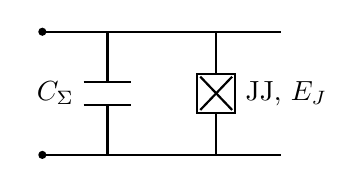
\begin{tikzpicture}[scale=0.92]
      \draw[thick] (-1.65,0.85)--(1.65,0.85);
      \draw[thick] (-1.65,-0.85)--(1.65,-0.85);
      \fill (-1.65,0.85) circle (1.6pt);
      \fill (-1.65,-0.85) circle (1.6pt);

      % Shunt capacitor
      \draw[thick] (-0.75,0.85)--(-0.75,0.16);
      \draw[thick] (-1.08,0.16)--(-0.42,0.16);
      \draw[thick] (-1.08,-0.16)--(-0.42,-0.16);
      \draw[thick] (-0.75,-0.16)--(-0.75,-0.85);
      \node[left] at (-1.08,0) {$C_\Sigma$};

      % Josephson junction: nonlinear inductive element
      \draw[thick] (0.75,0.85)--(0.75,0.27);
      \draw[thick,fill=white] (0.49,-0.27) rectangle (1.01,0.27);
      \draw[thick] (0.53,-0.23)--(0.97,0.23);
      \draw[thick] (0.53,0.23)--(0.97,-0.23);
      \draw[thick] (0.75,-0.27)--(0.75,-0.85);
      \node[right] at (1.02,0) {JJ, $E_J$};
    \end{tikzpicture}

    \vspace{-0.3em}
    \[
      H_{\mathrm{LC}}=\frac{Q^2}{2C}+\frac{\Phi^2}{2L},
      \qquad E_{m+1}-E_m=\hbar\omega.
    \]
    A linear inductance gives a quadratic potential and equal level spacing.
    Replacing the linear inductor with a Josephson junction gives
    \[
      H=4E_C(\hat n-n_g)^2-E_J\cos\hat\phi .
    \]
    The cosine potential makes the level spacing unequal.

    \column{0.51\textwidth}
    \centering
    \textbf{Josephson potential and energy levels}

    \begin{tikzpicture}[x=0.92cm,y=1.12cm,>=Stealth]
      \draw[->,gray] (-3.45,0)--(3.55,0) node[right] {$\phi$};
      \draw[->,gray] (0,-1.35)--(0,1.15) node[above] {$U(\phi)$};
      \draw[very thick,blue!70!black,domain=-3.15:3.15,samples=100]
        plot (\x,{0.9*(1-cos(\x r))-1.05});
      \node[blue!70!black,above right] at (1.95,0.55) {$-E_J\cos\phi$};

      \draw[very thick,blue!75!black] (-0.80,-0.72)--(0.80,-0.72)
        node[right] {$|0\rangle$};
      \draw[very thick,orange!90!black] (-1.13,-0.08)--(1.13,-0.08)
        node[right] {$|1\rangle$};
      \draw[very thick,gray!75!black] (-1.42,0.43)--(1.42,0.43)
        node[right] {$|2\rangle$};

      \draw[<->,thick] (2.35,-0.70)--(2.35,-0.10)
        node[midway,right] {$\hbar\omega_{01}$};
      \draw[<->,thick] (2.35,-0.06)--(2.35,0.41)
        node[midway,right] {$\hbar\omega_{12}$};
    \end{tikzpicture}

    \vspace{-0.4em}
    \[
      \omega_{12}\neq\omega_{01},\qquad
      |0\rangle\equiv\text{ground state},\quad
      |1\rangle\equiv\text{first excited state}.
    \]
    \small The unequal transition frequencies let a resonant microwave pulse
    address the qubit transition while limiting excitation of $|2\rangle$.
  \end{columns}
\end{frame}
